% ══════════════════════════════════════════
%  CHAPITRE 5 — SPRINT 2
% ══════════════════════════════════════════
\chapter{Sprint 2 « Analyses \& Déploiement »}

\section{Introduction}
Dans ce second sprint, nous nous concentrons sur l'exploitation et le traitement des données collectées : calcul de statistiques avancées, détection d'alertes automatiques, et déploiement du projet sur des serveurs Cloud (Astronomer).

\section{Objectif attendu et identification des tâches}

\subsection{Objectif attendu}
Mettre en place les analyses automatisées avec Apache Airflow et finaliser le déploiement complet de la plateforme pour la rendre accessible aux utilisateurs.

\subsection{Sprint Backlog}
\begin{itemize}
    \item \textbf{US7 :} Développement des DAGs d'analyse (corrélations, statistiques annuelles et mensuelles).
    \item \textbf{US8 :} Système d'alerte sur les pics de température et correction globale de bugs.
    \item \textbf{US9 :} Déploiement final sur Astronomer Cloud, tests finaux et rédaction de la documentation.
\end{itemize}

\section{Analyse détaillée des besoins}

\subsection{Diagramme de cas d'utilisation}
\begin{figure}[H]
\centering
\imgplaceholder{Figure~\ref{fig:uc_sprint2}}{Diagramme de cas d'utilisation du Sprint 2}
\caption{Diagramme de cas d'utilisation — Sprint 2}
\end{figure}

\subsection{Descriptions textuelles}
\textbf{Cas d'utilisation « Visualiser les statistiques »} : L'analyste choisit une période sur l'interface. Le système calcule les corrélations de Pearson en base de données et génère un graphique (Heatmap) interactif.

\textbf{Cas d'utilisation « Détecter un pic de chaleur »} : Le pipeline Airflow tourne en arrière-plan tous les jours. S'il détecte une température anormalement haute par rapport à la moyenne, il enregistre une alerte qui sera affichée automatiquement à l'utilisateur sous forme de notification.

\section{Prototypes d'interfaces}
\begin{figure}[H]
\centering
\imgplaceholder{Figure — Maquette Analyses}{Maquette de la page d'analyse}
\caption{Maquette de la page des analyses statistiques}
\end{figure}

\section{Modélisation conceptuelle}

\subsection{Diagramme de classes}
\begin{figure}[H]
\centering
\imgplaceholder{Figure~\ref{fig:class_diagram}}{Diagramme de classes des tables d'analyses}
\caption{Diagramme de classes — Analyses statistiques}
\end{figure}

\subsection{Diagrammes de séquence}
\begin{figure}[H]
\centering
\imgplaceholder{Figure~\ref{fig:seq_alert}}{Diagramme de séquence de la détection d'alertes}
\caption{Diagramme de séquence — Détection et affichage des alertes}
\end{figure}

\subsection{Diagramme d'activité}
\begin{figure}[H]
\centering
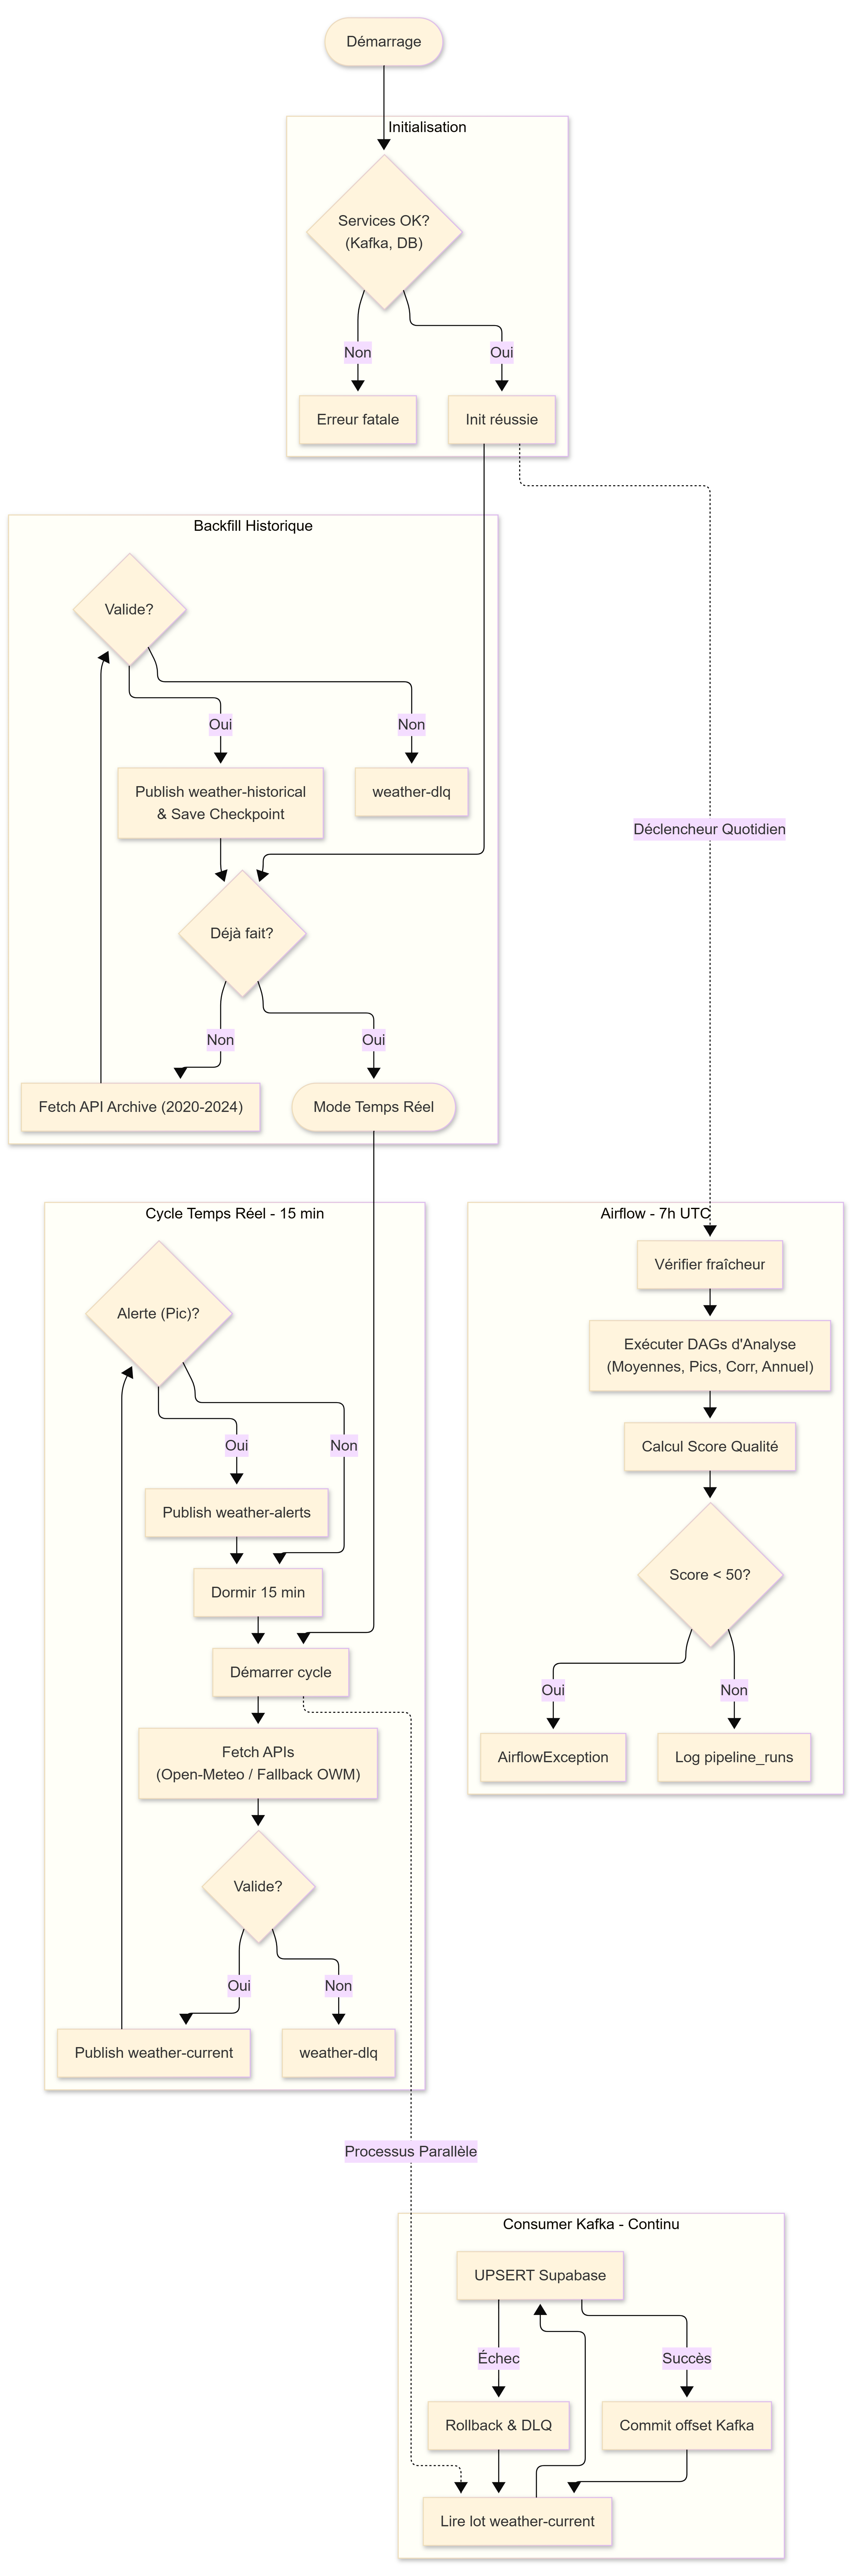
\includegraphics[width=\textwidth]{figures/activite.png}
\caption{Diagramme d'activité — Pipeline}
\end{figure}

\subsection{Diagramme de déploiement}
\begin{figure}[H]
\centering
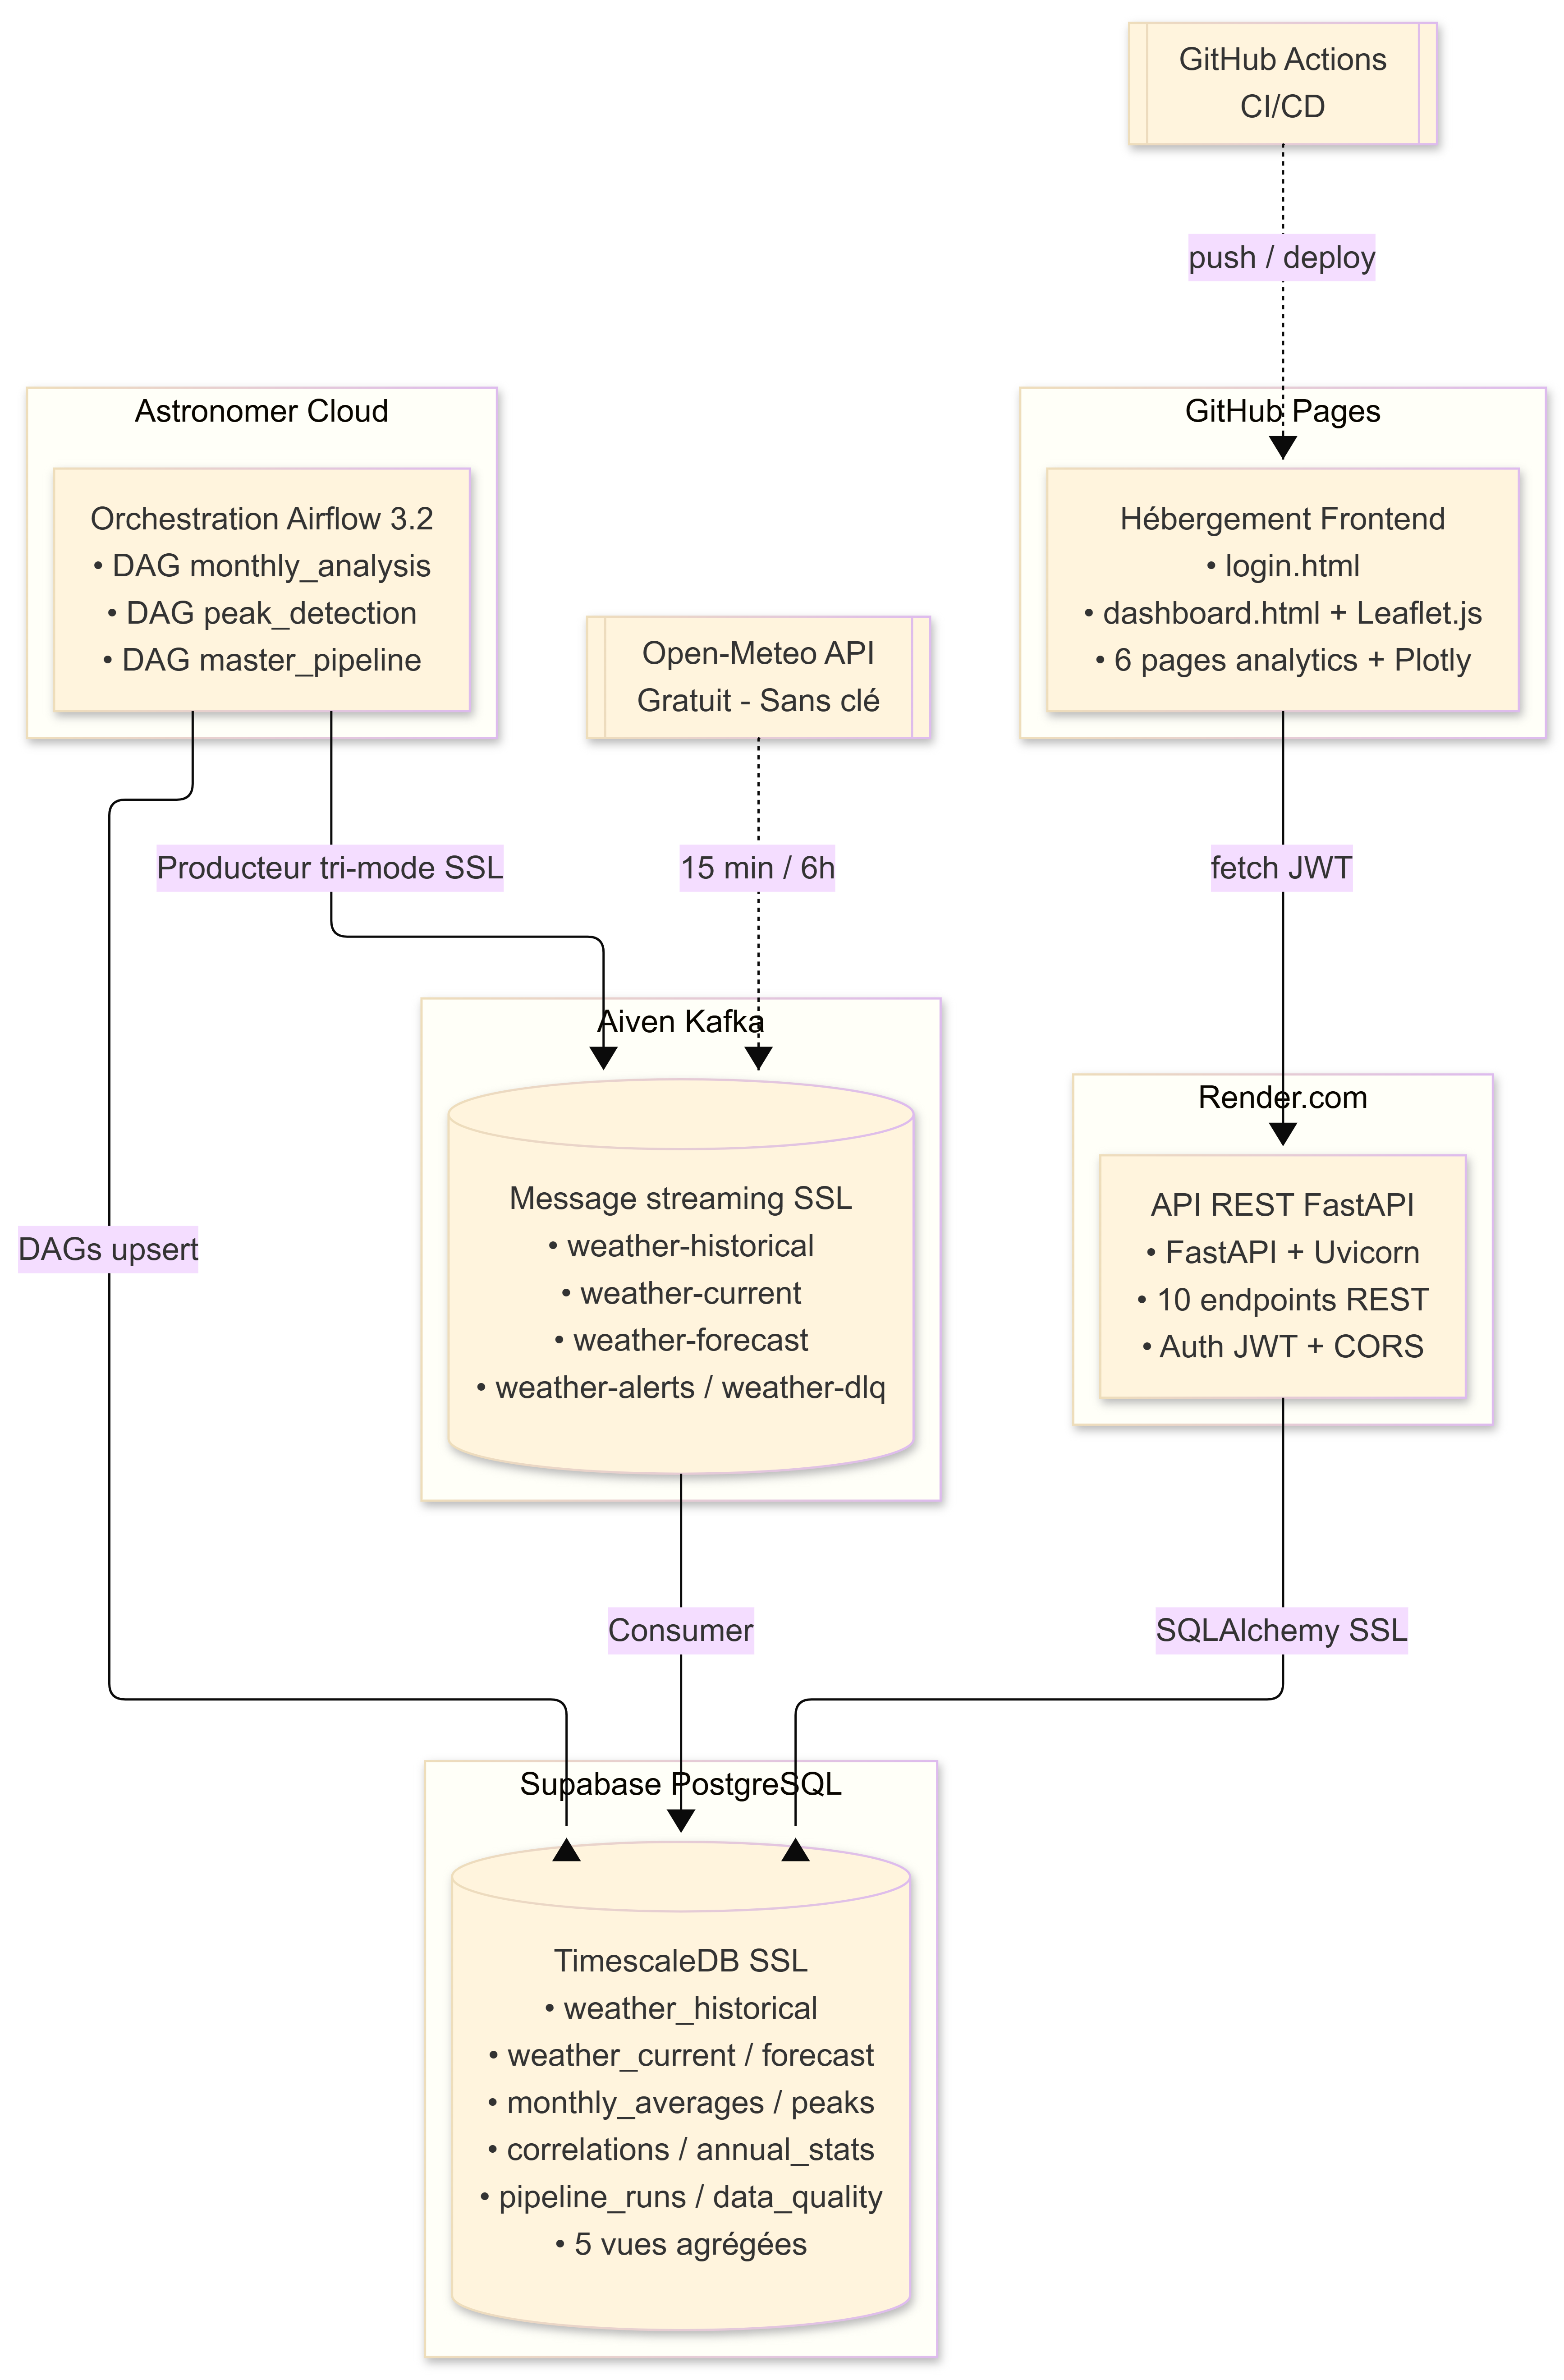
\includegraphics[width=\textwidth]{figures/deploiment.png}
\caption{Diagramme de déploiement}
\end{figure}

\section{Réalisation}
\subsection{Capture d'écran}
\begin{figure}[H]
\centering
\imgplaceholder{Figure~\ref{fig:airflow_ui}}{Capture de l'interface Airflow Astronomer}
\caption{Déploiement des DAGs sur l'environnement Cloud Airflow}
\end{figure}

\section{Tests et validations}
Les algorithmes statistiques développés ont été testés avec succès et l'orchestration avec Airflow fonctionne de manière 100\% automatisée sur le Cloud, respectant le planning d'exécution prévu.

\section{Conclusion}
Ce deuxième et dernier sprint finalise le projet. L'application est maintenant complète, fonctionnelle, déployée sur le Cloud, et répond parfaitement aux exigences techniques et fonctionnelles fixées dès le départ.
